% !TEX root=/home/tavant/these/manuscript/src/manuscript.tex



\section{Propulsion system for spacecrafts}
\label{sec-propulsion}
% \addcontentsline{toc}{section}{Propulsion system for spacecrafts}


In order to move in space, satellites, scientific probes, and spacecrafts in general rely on a propulsion system.
The cost to go from one location to another can be expressed as $\Delta v$, a measure of impulse needed to maneuver.
\nomenclature[Q]{$\Delta v$}{Measure of impulse needed for a space manoeuvre}
\Cref{fig-subway_DV} illustrates the $\Delta v$ required to evolve in the solar system.
We can see that reaching \ac{LEO} needs a $\Delta v$ of 9400 m/s while the \ac{GEO} is 3910 m/s further.
Landing on the Moon from the Earth ground requires a total of 15 km/s, while landing on Neptune requires $\Delta v =43.7$\,km/s.
For a spacecraft of instantaneous mass $M(t)$, with a propulsion system generating a thrust $T(t)$, the $\Delta v$ between $t_1$ and $t_2$ is
\begin{equation} \label{eq-dv}
  \Delta v = \int_{t_1}^{t_2} \frac{ \norm{T(t)}}{M(t)} dt.
\end{equation}
As expected, we see from \cref{eq-dv} that for a more massive spacecraft, a more intense, or a longer thrust is needed in order to obtain the same $\Delta v$.
\nomenclature[Q]{\ensuremath{ t}}{Time}
\nomenclature[Q]{\ensuremath{ T}}{Thrust}
\nomenclature[Q]{\ensuremath{ M}}{Mass of a spacecraft}
\begin{figure}[!hbt]
  \centering
  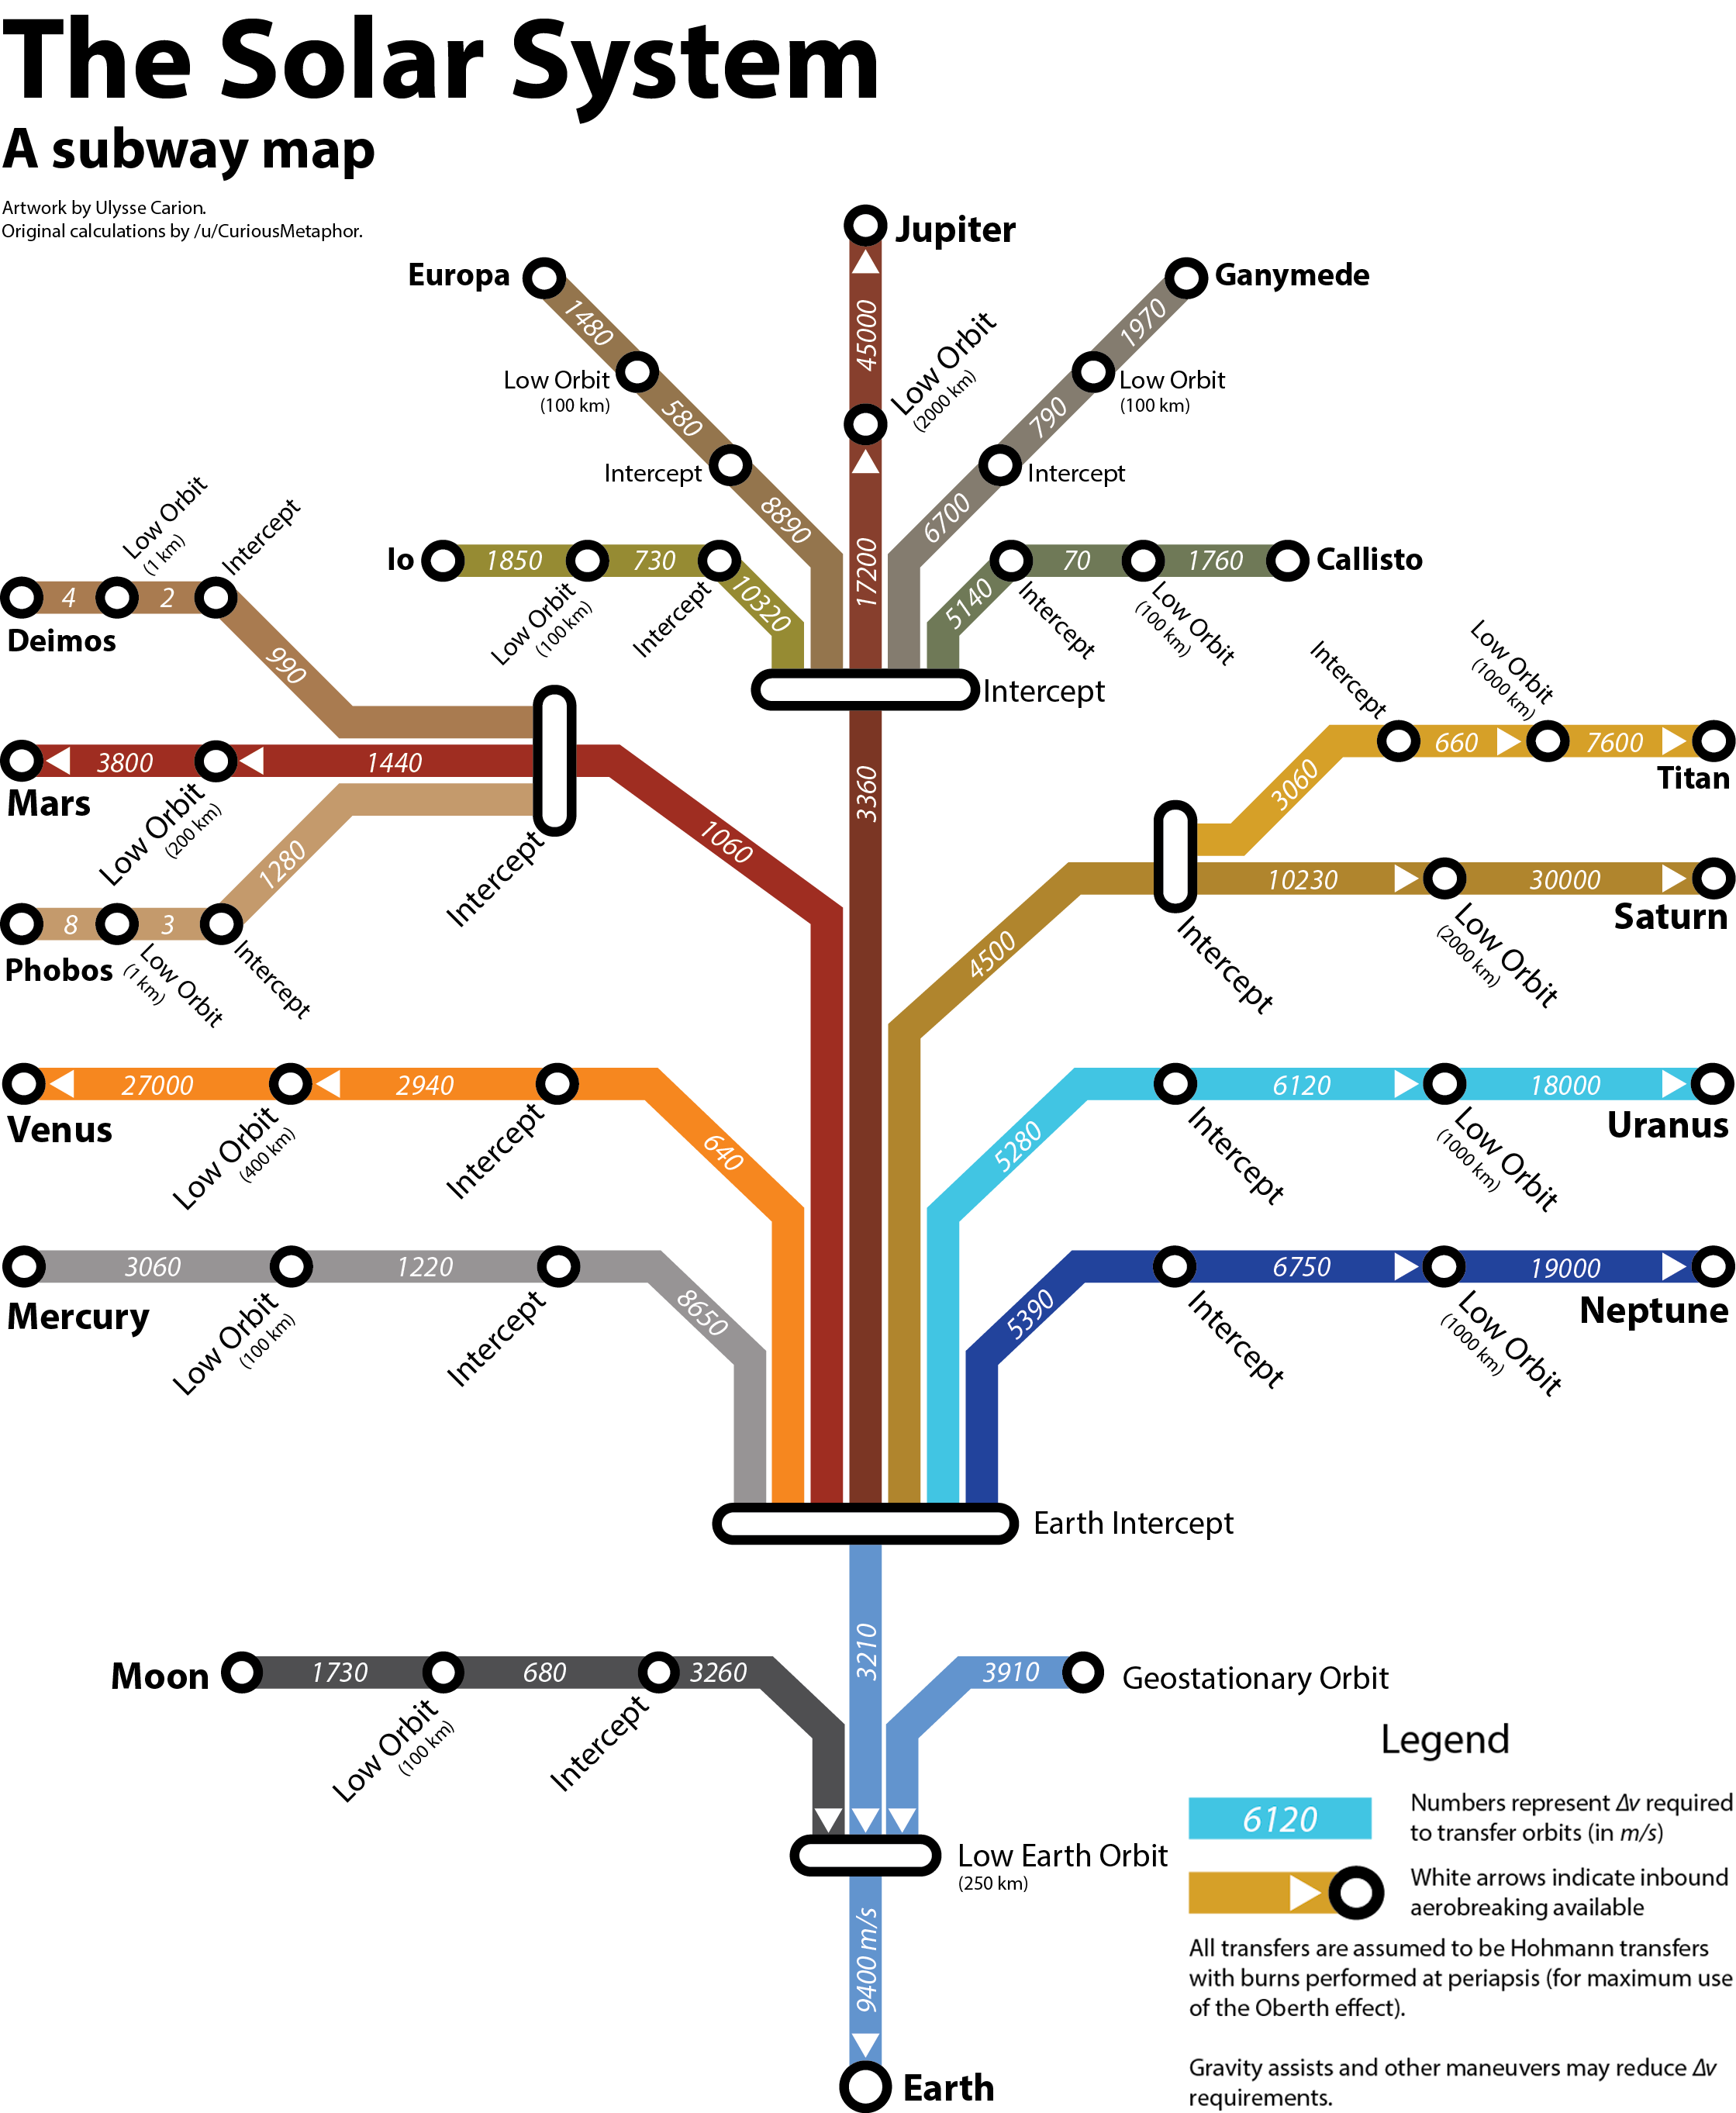
\includegraphics[width=\textwidth]{subway_map_legend}
  \caption{Representation of the different $\Delta v$ needed to go around the solar system, from \citet{reddit-subway}}
  \label{fig-subway_DV}
\end{figure}

\subsection{The rocket equation}
The thrust $T$ generated by ejecting mass at high velocity is
\begin{equation} \label{eq-thurst}
  T = v_{\rm ex} \dot{M}
\end{equation}
with $v_{\rm ex}$ the exhaust velocity of the propellant, and $\dot{M}$ the propellant mass flow rate through the thruster.
Hence,
\begin{equation} \label{eq-rocket}
  \Delta v = \int_{t_1}^{t_2} v_{\rm ex} \frac{ \norm{\dot{M}}}{M(t)} dt = v_{\rm ex} \ln \lp \frac{M_0}{M_1} \rp
\end{equation}
with $M_0 = M(t_0)$ and $M_1=M(t_1)$, and supposing that $v_{\rm ex}$ is constant.
We see from \cref{eq-rocket} that for a spacecraft of dry mass $M_1$ to have a given $\Delta v$, the exhaust velocity is directly linked to the initial \emph{wet} mass $M_0 = M_1 + M_{\rm prop}$, with $M_{\rm prop}$ the propellant mass.
\Cref{eq-rocket} is known as the rocket equation, or Tsiolkovsky's equation.
Usually, instead of the exhaust velocity $v_{\rm ex}$, the specific impulse ${\Isp} = g_0 v_{\rm ex}$, with $g_0$ the standard gravity, is used.
\nomenclature[Q]{\ensuremath{ \Isp}}{ Specific impulse, related to the exhaust velocity of a propellant}
\nomenclature[P]{\ensuremath{ g_0}}{  Standard acceleration due to gravity \nomunit{9.80665 m/s$^2$}}

\subsection{Chemical propulsion systems}
The usual rocket thruster uses a chemical reaction to generate the thrust.
For instance, the Vulcain (the thruster engine of the main stage of the European Ariane 5 and 6, developed by ArianeGroup, ex. Safran) uses the oxygen-hydrogen combustion, the most efficient chemical reaction for chemical thrusters \citep{nasa-H2O2}
\begin{equation*}
  2 {\rm H_2} + { \rm O_2} = 2 {\rm H_2 O} + 572 \text{~kJ},
\end{equation*}
with the energy of $572\,\kilo\joule$ of heat generated by $1\,\mole$ of oxygen.
This means that burning $1\,\kilo\gram$ of hydrogen-oxygen mixture generates a total energy of $13\,\mega\joule$. 
Supposing that the entire energy is converted into the exhaust of the water produced, its velocity would be of $5.1 \,\kms$.
In reality, the exhaust velocity of the Vulcain is of $4.2 \,\kms$, corresponding to $\Isp=431 \,\second$.
The efficiency of the Vulcain is close to 80\%, which is a very high efficiency, and it would be difficult to increase it significantly. 

In chemical propulsion systems, the fact that the energy released is related to the propellant mass gives an upper limit of exhaust velocity for a given combustion.
Electric propulsion engines, on the other hand, decouple the mass ejected (the propellant) from the energy source.
This decoupling allows a theoretical unlimited exhaust velocity.
Another advantage is the absence of reactive species, which lowers the security requirements impacting the spacecrafts.
Unfortunately, electric propulsion engines only work in vacuum and do not deliver sufficient thrust to compensate the earth gravity.
Hence, while electric propulsion can be used on spacecrafts, chemical propulsion is the only solution for rockets.

\subsection{Electric propulsion systems} \label{subsec-EP}
\ac{EP} systems mostly rely on plasmas \citep{charles2009,mazouffre2016}.
They have been successfully used since the 1960s by governments, but their complexity, the limited electric power available, and the inherent risk aversion of the space industry kept the \ac{EP} technologies hidden from the commercial applications \citep{lev2019}.
The breakthrough came in the '90s when the former Soviet Union's companies licensed the technology to Western propulsion companies.
However, many commercial satellite manufacturers were skeptical, until the first decade of the 21st century, which brought strong evidence of the competitiveness of \ac{EP}.
The landmark of commercial use of \ac{EP} is the selling of four all-electric satellites for \ac{GEO} by Boeing in 2012, the first two of which were launched in March 2015.

The two leading \ac{EP} technologies used are
\begin{itemize}
  \item the \ac{HET}, also known as Stationary Plasma Thruster (SPT) in Russia
  \item the Gridded Ion Thruster (GIT), usually referred simply as Ion Thruster
\end{itemize}




 
 \paragraph{The Gridded Ion Thruster} is a plasma chamber closed at one end by two or more grids.
 The plasma source can be an emitting cathode, generating energetic electrons that ionize the propellant (usually Xenon), or a \ac{RF} source.
 The potential difference between the grids accelerates the ions.
 Another cathode is used to neutralize the ion beam.
 Compared to \ac{HET}s, it produces an ion beam with less divergence and a higher \Isp of the order of 3000 to 4000~s.
 \Cref{fig-iongridded} shows a picture of the ion thruster used for the BepiColombo mission toward Mercury.
 We see the neutralizing cathode, the accelerating grid, and the ion beam.
 
\begin{figure}[!hbt]
  \centering
  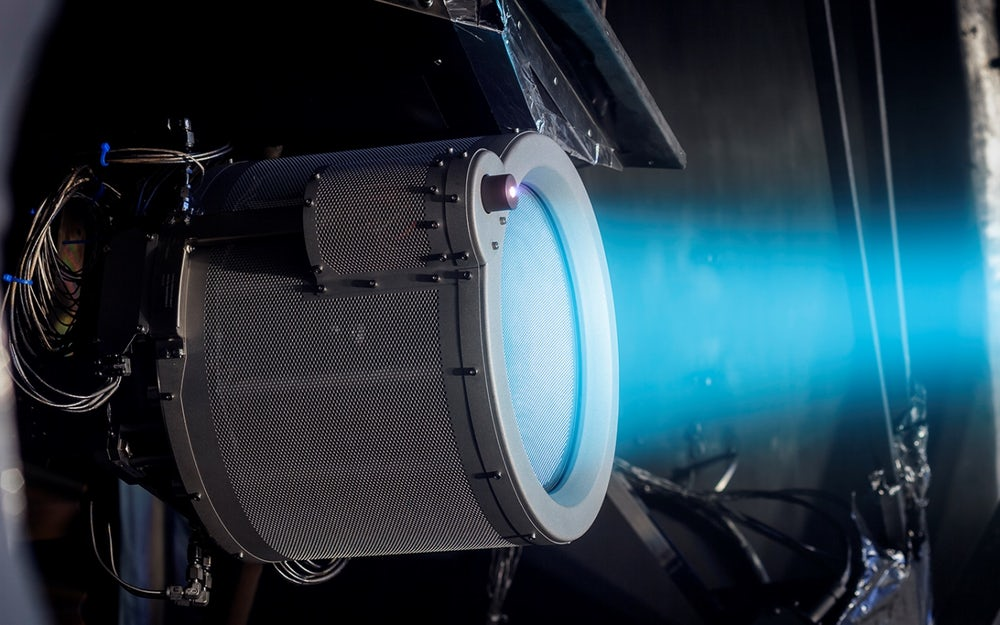
\includegraphics[width=\defaultwidth]{ion_Bepi.png}
  \caption{The T6 ion thruster will help send BepiColombo to Mercury. The neutralizing cathode is in the upper left quadrant of the thruster. (Credit\string: QinetiQ)}
  \label{fig-iongridded}
\end{figure}
 
 \paragraph{Hall Effect thrusters} use a magnetic barrier to both increase the ionization of the propellant and create the accelerating electric field.
 A detailed description of the \ac{HET} is presented in the next section.
 One cathode is used to start the discharge and neutralize the ion beam.
 Compared to GITs, \ac{HET}s need less power, hence reaching better thrust per power ratio and a smaller (therefore lighter) Power Processing Unit.
 Recently, the first satellites of two mega-constellations (OneWeb, 648 satellites planned, from which six were launched on February, \nth{26} 2019, and Starlink, 12~000 satellites planned, from which 62 were launched on May, \nth{23} 2019) were sent to Low Earth orbit, both using \ac{HET}s. 
 % Compared to GITs, \ac{HET}s need less power, and fewer power sources, hence reaching better thrust per power ratio and smaller (therefore lighter) Power Processing Unit. 
 Their typical \Isp is of the order of 1500~s.
 \Cref{fig-13kWHET} shows a high power prototype firing.
 We see the emitting cathode, in this design at the center, and the ion beam.
 \begin{figure}[!hbt]
   \centering
   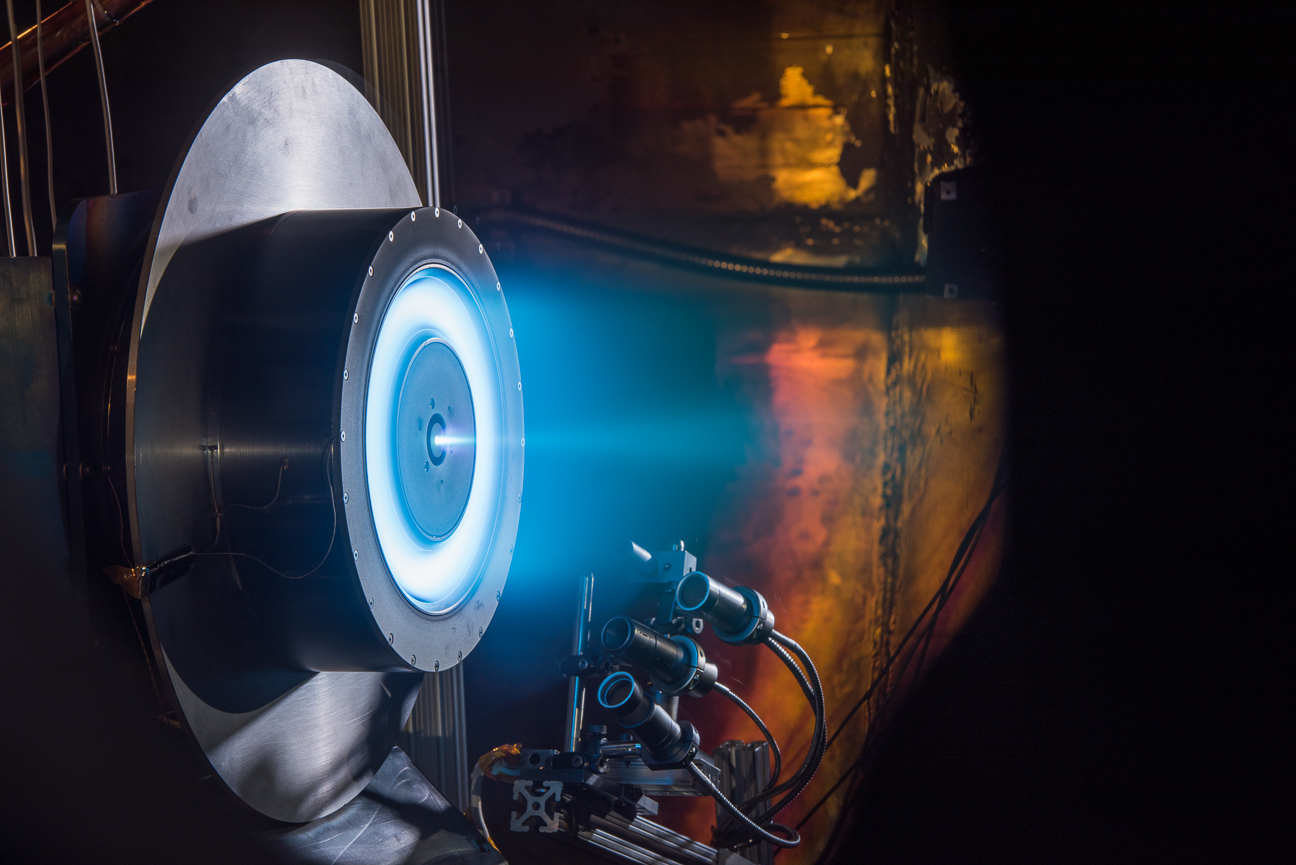
\includegraphics[width=\defaultwidth]{HET_X3_light.png}
   \caption{A 13 kilowatt \acs{HET} prototype on a testing bench in a vacuum chamber (Credit\string: NASA).  }
   \label{fig-13kWHET}
 \end{figure}
 
 
 \subsection{Electric propulsion environment in France} \label{subsec-HET_thruster}
 
 France is a leader country in the aerospace industry in both Europe and the world, with companies such as  Airbus, Thales, Safran, and ArianeGroup (join-venture of Safran and Airbus).
 As a consequence, the French ecosystem of electric propulsion is vibrant.
 The main thrusters produced in France are the PPS series by Safran, with the \PPS1350 (version G at 1.5~kW nominal power, and the version E at 2.7~kW), and the \PPS5000, a high power \ac{HET} at 5~kW, the first models of which have been delivered to Boeing in May 2019.
 A low-power version (between 500W and 1kW) of the \PPS{}  is currently developed\citep{vaudolon2018}.
 A list for the \PPS{} series elements and their respective characteristics can be seen in \cref{tab-ppsfamily}.
 \begin{table}[!hbt]
 \ra{1.3}
   \centering
   \caption{Members of the \PPS{} series developed by Safran Aircraft Engines \citep{boniface2017,duchemin2017,vaudolon2018}. The nominal operating condition of the \PPS{X00} is not fixed yet.}
   \label{tab-ppsfamily}
   \begin{tabular}{@{}llll@{}} \toprule
   Name & Power & Thrust & \Isp \\ \midrule
   \PPS1350-G & 1.5~kW & 89~mN  & 1650~s \\
   \PPS1350-E & 2.7~kW & 140~mN  & 1800~s \\
   \PPS5000 & $3-5$~kW & $150-300$~mN  & $1850-1700$~s \\
   \PPS{X00} & $\sim 650$W &  $\sim$40~mN & $\sim 1450$~s \\
   \bottomrule
   \end{tabular}
 \end{table}
 
 Several initiatives concerning the small-sat sector are also undertaken, such as the start-ups Exotrail (micro \ac{HET}) and Thrust Me (radio frequency Ion Thruster), or the Electron Cyclotron Resonance Thruster at ONERA.
 Since 1996, numerous research projects have been carried out in France on HET with  the \ac{CNES}, SAFRAN and several research laboratories: ICARE, LAPLACE, CPHT, LPP, etc. \citep{boniface2017}.
 These numerous actors, combined with the support of the French and European space agencies, compose a stimulating environment that contributes both to the most mature technologies and the promising \ac{EP} concepts that could disrupt the propulsion sector.
 